\documentclass[draft,linenumbers]{agujournal2018}
\usepackage{apacite}
\usepackage{url} %this package should fix any errors with URLs in refs.
\usepackage{amsmath}

%%%%%%%
%\usepackage{trackchanges}
% uncomment the line above to use the TrackChanges package to mark revisions if needed.
% The trackchanges package adds five new LaTeX commands:
%
%  \note[editor]{The note}
%  \annote[editor]{Text to annotate}{The note}
%  \add[editor]{Text to add}
%  \remove[editor]{Text to remove}
%  \change[editor]{Text to remove}{Text to add}
%
% complete documentation is here: http://trackchanges.sourceforge.net/
%%%%%%%

\draftfalse

\journalname{Space Weather}

\begin{document}
\title{A Test of the Frequency Independence Assumption of the Power System Parameters used in Geomagnetically Induced Current Calculations}

\authors{R.S. Weigel\affil{1} and P.J. Cilliers\affil{2}}

\affiliation{1}{Space Weather Lab, George Mason University}
\affiliation{2}{South African National Space Agency}

\affiliation{1}{4400 University Drive, Fairfax VA 22030}
\affiliation{2}{Hospital Street, Hermanus 7200}

\correspondingauthor{R.S. Weigel}{rweigel@gmu.edu}

\begin{keypoints}
\item The power system parameters derived from GIC and geoelectric field measurements are frequency dependent.
\item A GIC prediction model with frequency dependence significantly outperforms a frequency independent model.
\item The best predictions are found when the model input is not the measured geoelectric field but rather the geoelectric field predicted by a transfer function model driven by the geomagnetic field.
\end{keypoints}

\begin{abstract}
A common assumption used in estimating geomagnetically induced currents (GICs) in a power system given a direct measurement or indirect estimate (via a transfer function with input of the geomagnetic field) of the horizontal geoelectric field components $E_x$ and $E_y$ on Earth's surface is that the system is resistive. That is, the approximation $GIC(t)$  $=$ $a_oE_x(t) + b_oE_y(t)$ (Model 1) is used, where $a_o$ and $b_o$ are frequency independent network parameters.  We provide the first test of this assumption using GIC measurements made in a 187 kV transformer connected to a $\sim$100 km power line in Memanbetsu, Japan and geoelectric field measurements made at the Memanbetsu Magnetic Observatory $\sim$10 kilometers away.  We compute frequency dependent network parameters  $A(\omega)$ and $B(\omega)$ in Model 2, $GIC(\omega)$ $=$ $A(\omega)E_x(\omega) + B(\omega)E_y(\omega)$, and find that they are frequency dependent and that this model provides a significantly better representation of measured GIC.
\end{abstract}

\section{Introduction}

Geomagnetically induced currents (GICs) are electric currents in man-made conducting systems due to electric fields induced near Earth's surface. These fields are a result of time variations in ionospheric currents on timescales on the order of hours \citep{Ohtani2000} and the movement of Earth's surface relative to slow-varying current systems in Earth's ionosphere that are near stationary relative to the Sun \citep{Stening2013}. Of particular interest are currents induced in electric power systems as they can lead to system degradation, disruption, and failure \citep{Albertson1993,NERC2012}. Accurate estimation of GICs given direct measurements of the electric field (or estimates based on the geomagnetic field) is important for power system design, retrospective analysis, and for the mitigation of the impacts of space weather on power systems [REFS].

A common assumption made in estimates of GIC using either measured or estimated values of the horizontal geoelectric field at Earth's surface, $\mathbf{E}$, is that the power system is resistive or quasi-DC so that the relationship $GIC(t) = a_oE_x(t) + b_oE_y(t)$ holds \citep{Albertson1981,Lehtinen1985}.  The coefficients $a_o$ and $b_o$ can then be calculated analytically using information about the connectivity of the power lines and values of the conductor and transformer resistances using DC circuit methods \citep[e.g.][]{Boteler2014a,Boteler2014b}. This assumption has been used or stated in many works, for example, \citet{Pulkkinen2007,Wik2008,Pulkkinen2010,Ngwira2011,Viljanen2012,Overbye2012}.

In this work, we use a unique dataset in which measurements $\mathbf{E}$ and the surface horizontal geomagnetic field, $\mathbf{B}$, were made near a site where GICs were being measured in an electric power system.  We first estimate the system parameters $a_o$ and $b_o$ using conventional methods, which assume that they are frequency independent.  Then, we use a model in which the system parameters are frequency dependent, compute the frequency dependence, and compare this model with the traditional frequency independent model. 

\section{Data}

The 1-second-cadence GIC data used in this paper span a total of 35 days across the 10 intervals: 2006-04-03 -- 2006-04-10, 2006-07-25 -- 2006-07-29, 2006-08-05 -- 2006-08-08, 2006-08-19 -- 2006-08-21, 2006-11-07 -- 2006-11-12, 2006-11-28 -- 2006-11-29, 2006-12-01, 2006-12-14 -- 2006-12-15, 2007-11-18 -- 2007-11-20, and 2007-11-22 -- 2007-11-22 that have been presented previously in \citet{Watari2009} and \cite{Watari2015}.

One-second-cadence geoelectric field and geomagnetic field data from Kakioka Magnetic Observatory were obtained from the Japan Meteorological Agency data portal. Data for the longest continuous time span, 2006-04-02 through 2006-04-10 are shown in the top and middle panels of Figure~\ref{sample}.

Unphysical spikes in the electric field measurements assumed to be unphysical when the absolute value of a component $i$ of the electric field changed by more than 1 mV/km at time $t_s$, and the values $E_i(t_s-2)$ through $E_i(t_s+4)$ were replaced using linear interpolation of the values at $E_i(t_s-3)$ and $E_i(t_s + 5)$. In the sample shown in Figure~\ref{sample}, 21 spikes were identified in $E_x$ and zero in $E_y$.

The only modifications made to the magnetic field measurements was the replacement of 36 data points in all components of the magnetic field on 2006-08-06 with linearly interpolated values. The values for $E_x$ and $E_y$ were the same and much larger than the surrounding values.

The GIC dataset includes 1-second raw data and 1 Hz low-pass filtered raw measurements.  The results presented here are for the 1 Hz low-pass filtered GIC values and data for the time interval 2006-04-02 through 2006-04-10 is shown in the bottom panel of Figure~\ref{sample}.

The GIC data contains non-physical spikes that are followed by a relaxation time of approximately 80 seconds. These spikes were removed by identifying times $t_s$ when the change in $|GIC|$ was greater than $0.04$ Amps and then data in a window $GIC(t_s-2)$ through $GIC(t_s+100)$ was replaced using a linear interpolation of the values at $GIC(t_s-3)$ and $GIC(t_s + 101)$. In the example interval shown in Figure~\ref{sample}, 493 spikes were removed.

\section{Models and Methods}

To determine the coefficients $a_o$ and $b_o$ in the frequency independent model, Model 1,

\begin{linenomath*}
\begin{equation}
G_o(t) = a_oE_x(t) + b_oE_y(t)
\label{model1}
\end{equation}
\end{linenomath*}

\noindent
we form the matrix equation $GIC = \underline{\mathbf{E}}\cdot\mathbf{p}$, where GIC is a 864000x1 matrix of observations, $\mathbf{p} = [a_o,b_o]^T$, and $\underline{\mathbf{E}}$ is a 86400x2 matrix with $N$ rows of $[E_x(t), E_y(t)]$ observations. The values of $\mathbf{p}$ are then obtained using a standard linear regression solver. The values of $a_o$ and $b_o$ determined in this way correspond to those that minimize the sum-of-squares of $GIC(t)-G_o(t)$ for all values of $t$. \citep[][ provided the mathematically equivalent closed-form equations.]{Pulkkinen2007}

In Model 2, we assume that the system parameters are frequency dependent

\begin{linenomath*}
\begin{equation}
G_E(\omega) = A(\omega)E_x(\omega) + B(\omega)E_y(\omega)
\label{model2}
\tag{2a}
\end{equation}
\end{linenomath*}

\noindent
In the time domain, this is equivalent to

\begin{linenomath*}
\begin{equation}
G_E(t) = \sum_{\tau=-\infty}^{\infty}\big[a(\tau)E_x(t-\tau) + b(\tau)E_y(t-\tau)\big]
\label{model2b}
\tag{2b}
\end{equation}
\end{linenomath*}

\noindent
were the parameters $a$ and $A$ and $b$ and $B$ are inverse fourier transforms of each other.

The third model considered uses the electric field $\mathbf{E}'$ in Equation~\ref{model1}, where $\mathbf{E}'$ was computed using the measured magnetic field and a transfer function $\mathbf{Z}$: $\mathbf{E}'(\omega) = \mathbf{Z}(\omega)\mathbf{B}(\omega)$:

\setcounter{equation}{2}
\begin{linenomath*}
\begin{equation}
G_{E'}(\omega) = A(\omega)E'_x(\omega) + B(\omega)E'_y(\omega)
\end{equation}
\end{linenomath*}

\noindent
where, explicitly, the electric field components are $E'_x$ = $Z_{xx}B_x + Z_{yx}B_y$ and $E'_y = Z_{yx}B_x + Z_{yy}B_y$. Substitution gives

\begin{equation*}
G_{E'}(\omega) = \big[A(\omega)Z_{xx}(\omega) + B(\omega)Z_{yx}(\omega) \big] B_x(\omega) + \big[ A(\omega)Z_{xy}(\omega) + B(\omega)Z_{yy}(\omega) \big] B_y(\omega)
\end{equation*}

That is, instead of using the measured electric field directly as in Model 2, we use a transfer function that relates $\mathbf{E}$ to $\mathbf{B}$ to provide an estimate of the electric field based on the magnetic field. In this work, we have computed $\mathbf{Z}$ using the method described later in this section; $A(\omega)$ and $B(\omega)$ are taken from the solution of Equation~\ref{model2}, using the method also described later in this section.

A fourth model was also considered:

\begin{linenomath*}
\begin{equation}
G_B(\omega) = Z_x(\omega)B_x(\omega) + Z_y(\omega)B_y(\omega)
\end{equation}
\end{linenomath*}

\noindent
In this model, the transfer function components $Z_x$ and $Z_y$ are determined directly from measurements of $GIC$ and $\mathbf{B}$ and is expected to produced predictions of $GIC$ that are similar to that obtained from Model 3.

The parameters in Model 2 and 4 can be computed using either a time or frequency domain method. In the time domain method, fixed values of the upper ($N_c$) and lower ($N_c$) limits are selected in the summations in Equation~\ref{model2b} (and equivalent for Equation 4) and then the equation is repeated for at least ($N_c+N_a+1$) time values and then the resulting over-determined set of equations is inverted to find the unknowns $a(\tau)$ and $b(\tau)$ for $N_a \le \tau \le Nc$.

In the frequency domain method, estimates of $A(\omega)$ and $B(\omega)$ are made at evaluation frequencies, $\omega_e$, by performing a least squares regression using Equation~\ref{model2} and a set $G_E(\omega)$ and $\mathbf{E}(\omega)$ values near $\omega_e$. To convert the frequency domain transfer functions $A(\omega)$ and $B(\omega)$ estimated at the frequencies $\omega_e$ to impulse responses $a(\tau)$ and $b(\tau)$, they are first linearly interpolated onto a 1 Hz frequency grid and then inverse fourier transformed. The transfer function magnitudes $|A(\omega)|$ and $|B(\omega)|$ were calculated by linear interpolation of the transfer function magnitudes (instead of linearly interpolating the real and imaginary components and then computing the magnitude). The same approach is used for solving for the transfer function $\mathbf{Z}$ in $\mathbf{E}(\omega) = \mathbf{Z}(\omega)\mathbf{B}(\omega)$ - the $xx$ and $yx$ components of $\mathbf{Z}$ are solved for using measured values of $E_x$, $B_x$, and $B_y$ in $E_x = Z_{xx}B_x + Z_{yx}B_{y}$, and the $yx$ and $yy$ components of $\mathbf{Z}$ are solved for using measured values of $E_y$, $B_x$, and $B_y$ in $E_y = Z_{yx}B_x + Z_{yy}B_y$. Additional details on the method are given in \cite[][and references therein.]{Weigel2017}.

It is expected that the time and frequency domain methods should give similar results because the transfer functions in the time- and frequency-domains are mathematically related \citep{Schoukens2004,Ljung2007}, although differences may exist as a result of implementation choices or roundoff \citep{Ljung2004}.  For example, regarding implementation, in the time domain method we choose a finite value of $N_c$ and $N_a$ and in the frequency domain method, we choose the set of evaluation frequencies $\omega_e$, an averaging window function, and $\omega$ values (which depend on the length of the time series used to calculate the spectra).

Because the frequency domain computations are significantly faster, the results presented here are based on the frequency domain results and only spot checks were performed to verify that the time- and frequency-domain methods gave consistent results.

Transfer function parameters were computed for each of the 35 unique 1-day window segments of available data. The average transfer function magnitude was obtained by averaging these 35 transfer function magnitudes; the average transfer function phase was obtained using the average real and imaginary components, respectively, of the 35 transfer functions. The average impulse response functions were obtained by averaging the 35 impulse response functions.

There are many statistical methods that have been proposed to estimate transfer functions in the magnetotelluric literature that use additional steps, processing, and assumptions \citep{Egbert1986,Chave1987,Chave1989,Jones1989,Larsen1996,Egbert1997,Eisel2001,Chave2004,Chave2012,Chave2017} beyond the ones used that follow the basic method in \cite{Simpson2005}. The additional steps and processing were developed to address leakage, un-removed data spikes and shifts, high levels of noise contamination, time intervals in which the model assumptions are violated, bias, and the fact that errors in the fits of the transfer function at each evaluation frequency may not be Gaussian distributed. These works typically involve the estimation of a robust and low bias transfer function. In the results presented, we did not use a robust statistical method to calculate the transfer function or a bias correction algorithm - our primary interest is comparing the ability of different models to predict the data (in a mean-squared-error sense) rather than estimating low-bias model parameters. As discussed in ~\cite{Weigel2017}, a model developed using robust and bias correction methods will not necessarily be an optimal prediction model.

However, several alternative methods for computing the transfer functions were tested individually by modifying the basic method described above to determine if there was a change in the computed transfer functions and each model's prediction ability. When using these alternative methods, we find that the conclusions made regarding the differences each model's prediction ability do not change, the differences in each model's prediction performance is within the calculated uncertainty of the used method, and the transfer function values are within the error bars of the used method when the signal to noise ratio is above $\sim$5. The experiments in this regard are discussed in the following section.

\section{Results}

The out-of-sample prediction metrics for each model on a given day was determined by computing the average model parameters using the remaining 34 days of data, generating a prediction time series on each of the 34 days using the average model parameters, and then computing the prediction metrics for each of the 34 days. This process was repeated to create a set of 35 out-of-sample prediction metrics for each model.

The performance of each model in predicting $GIC$ was assessed using three metrics: the prediction efficiency, PE, the mean-squared-error (MSE) ratio, and the signal-to-noise ratio. 

The prediction efficiency, PE, is the ``Case I'' skill score described by \cite{Murphy1988} and is defined as $PE$ = 1 - variance(Prediction Error)/variance(Predicted) and is a measure of the skill of the model relative to the variance in the data that are predicted, and it represents the fraction of the variance in the predicted data that predicted by the model.

The average PE and MSE ratio was computed by averaging the 35 PE and MSE ratios; the average signal-to-noise ratio at a given frequency is the average of the 35 signal-to-noise ratios at that frequency. The 95\% confidence interval, CI, on the PE and MSE ratio was calculated using 1000 bootstrap samples of the 35 prediction metrics. The typical difference between the limits when the confidence intervals were computed assuming the values were Gaussian-distributed was $\sim$2\%.

\begin{table}
\caption{Out-of-sample model performance metrics for models $m=1-4$. $MSE_m/MSE_1$ is the ratio of the MSE for model $m$ to that of Model 1. The PE and MSE ratios are the average of 35 values and the confidence interval, CI, was determined from 1000 bootstrap samples of these 35 values.}
\centering
\begin{tabular}{l c c c c}
\hline
$m$\hspace{1em} Model & PE & 95\% CI & MSE$_m$/MSE$_1$ & 95\% CI\\
\hline
1\hspace{1em} $G_o(t) = a_oE_x(t) + b_oE_y(t)$ & 0.35 & [0.25, 0.45] & 1.0 & \\
2\hspace{1em} $G_E(t) = A(\omega)E_x(t) + B(\omega)E_y(t)$ & 0.60 & [0.54, 0.65] & 1.8 & [1.6,2.0]\\
3\hspace{1em} $G_{E'}(t) = A(\omega)E'_x(t) + B(\omega)E'_y(t)$ & 0.78 & [0.76, 0.80] & 3.1 & [2.8,3.4]\\
4\hspace{1em} $G_{B}(t) = Z_xB_x(t) + Z_yB_y(t)$ & 0.83 & [0.80, 0.85] & 4.6 & [3.8,5.3]\\
\hline
\end{tabular}
\end{table}

Figure~\ref{predictions} shows a 1-day interval for which the value of the prediction efficiency for each model was in the same order as that shown in Table~1, i.e., Model 4 has the highest PE and Model 1 has the lowest.

The primary conclusions of this work follow from the results shown in Table~1: the frequency dependent model, Model 2, is significantly better at predicting GIC than the frequency independent model, Model 1. Model 3, which uses magnetic field measurements as in input provides better estimates of $GIC$ than Model 2. Model 4, in which a transfer function that connects $GIC$ to $\mathbf{B}$ was derived directly from the data, provides the best predictions of $GIC$.

Figure~\ref{SN} shows the average signal-to-noise ratios as a function of period for the four models. The error bars represent one standard error of the 35 SN ratios at each period. Consistent with the results in Table~1, the SN ratio for Model 1 is consistently lower than that for Models 2-4.  Above $1400$~s (24~min), the SN ratio ordering is consistent with the PE and MSE ratios shown in Table~1. Below $500$~s (8~min), Model 2 has the largest SN ratio. This result is somewhat visible in the sample interval shown in Figure~\ref{predictions} - at approximately 2006-08-07 07:00, the high frequency fluctuations in the prediction error for Model 2 are smaller than that for Models 3 and 4.

The average parameters for Model 1 are $a_o =$ $71.9 \pm 27.8$ A/(V/km) and $b_o =$ $-70.0 \pm 65.8$ A/(V/km) and the distribution of the 35 parameters calculated using each 1-day interval is shown in Figure~2. The wide distribution and large error bars are suggestive that the model is a poor representation of the measurements. However, the model does have a good prediction performance - the PE is 0.35 and the data/model correlation coefficient of 0.64. In a similar way that $|\mathbf{B}(t)|$ or $d|\mathbf{B}(t)|/dt$ are often good predictors of $GIC(t)$ [REFS] despite the fact that physically $\mathbf{E}$ drives $GIC$ and $\mathbf{E}$ is related to $\mathbf{B}$ through a frequency dependent transfer function, Model 1 is a fair predictor of $GIC$, but is a poor approximation relative to Models 2 and 3. For the data considered in this work, when a model $G(t) = c_oB_x(t) + d_oB_y(t)$ is used, were $c_o$ and $d_o$ are constants, the in-sample average prediction efficiency is comparable to that of Model 1, but the out-of-sample prediction efficiency is negative.

The average parameters for Models 2 and 4 are shown in Figure~\ref{H}--\ref{Phi}. The error bars at each time step or period is the standard error of the 35 values used to compute the average. 

Figure \ref{H} shows that the timescale of variations of an impulse in $\mathbf{E}$ for Model 2 and $\mathbf{B}$ for Model 4 are similar and are different from zero at more than one time value (the impulse response for Model 3 is similar to that of Model 2 and is not shown). By definition, the impulse response for Model 1 is zero except at $t=0$. Note that the sign of the impulse response at $t=0$ is opposite for Model 1 and Model 2 for the $E_y$ coefficient - at $t=0$, $b_o < 0$ while $b(0)>0$.

Figure~\ref{Z} shows that the frequency domain transfer functions for Model 2 vary by an order of magnitude on timescales of 60 seconds to 12 hours (that for Model 1 is constant by definition). For this system, GIC is most dependent on $E_y$, which has less variability than $E_x$ - the variance in $E_x$ is $\sim$5x larger than $E_y$ over the entire dataset (this is also visible in Figure~\ref{sample}). 

Figure~\ref{Phi} shows the transfer function phases. By definition, that for Model 1 is zero.

Several of these methods were tested individually by modifying the method described above to determine their impact on the computed transfer functions and their over all results. 

\begin{itemize}
\item Using robust regression (with either bi-square or Huber weighting) instead of linear regression when computing the transfer function estimates at each $\omega_e$

\item Averaging the 35 transfer functions using the Huber M-estimator with a $\psi$-function \citep{Huber2011}. 

\item Using weighted averages of the 35 transfer functions with the weighting at each frequency equal to the in-sample coherence at that frequency

\item Windowing the signals in the frequency domain using a rectangular window (instead of Parzen)
\end{itemize}

\section{Discussion and Conclusions}


\acknowledgments
Magnetic and electric field data made at the Kakioka Magnetic Observatory was obtained from the Japan Meteorological Agency data portal \url{http://www.kakioka-jma.go.jp/obsdata/metadata/en}. GIC data provided by ...

\bibliography{paper.bib}


\clearpage

\begin{figure}[h]
\centering
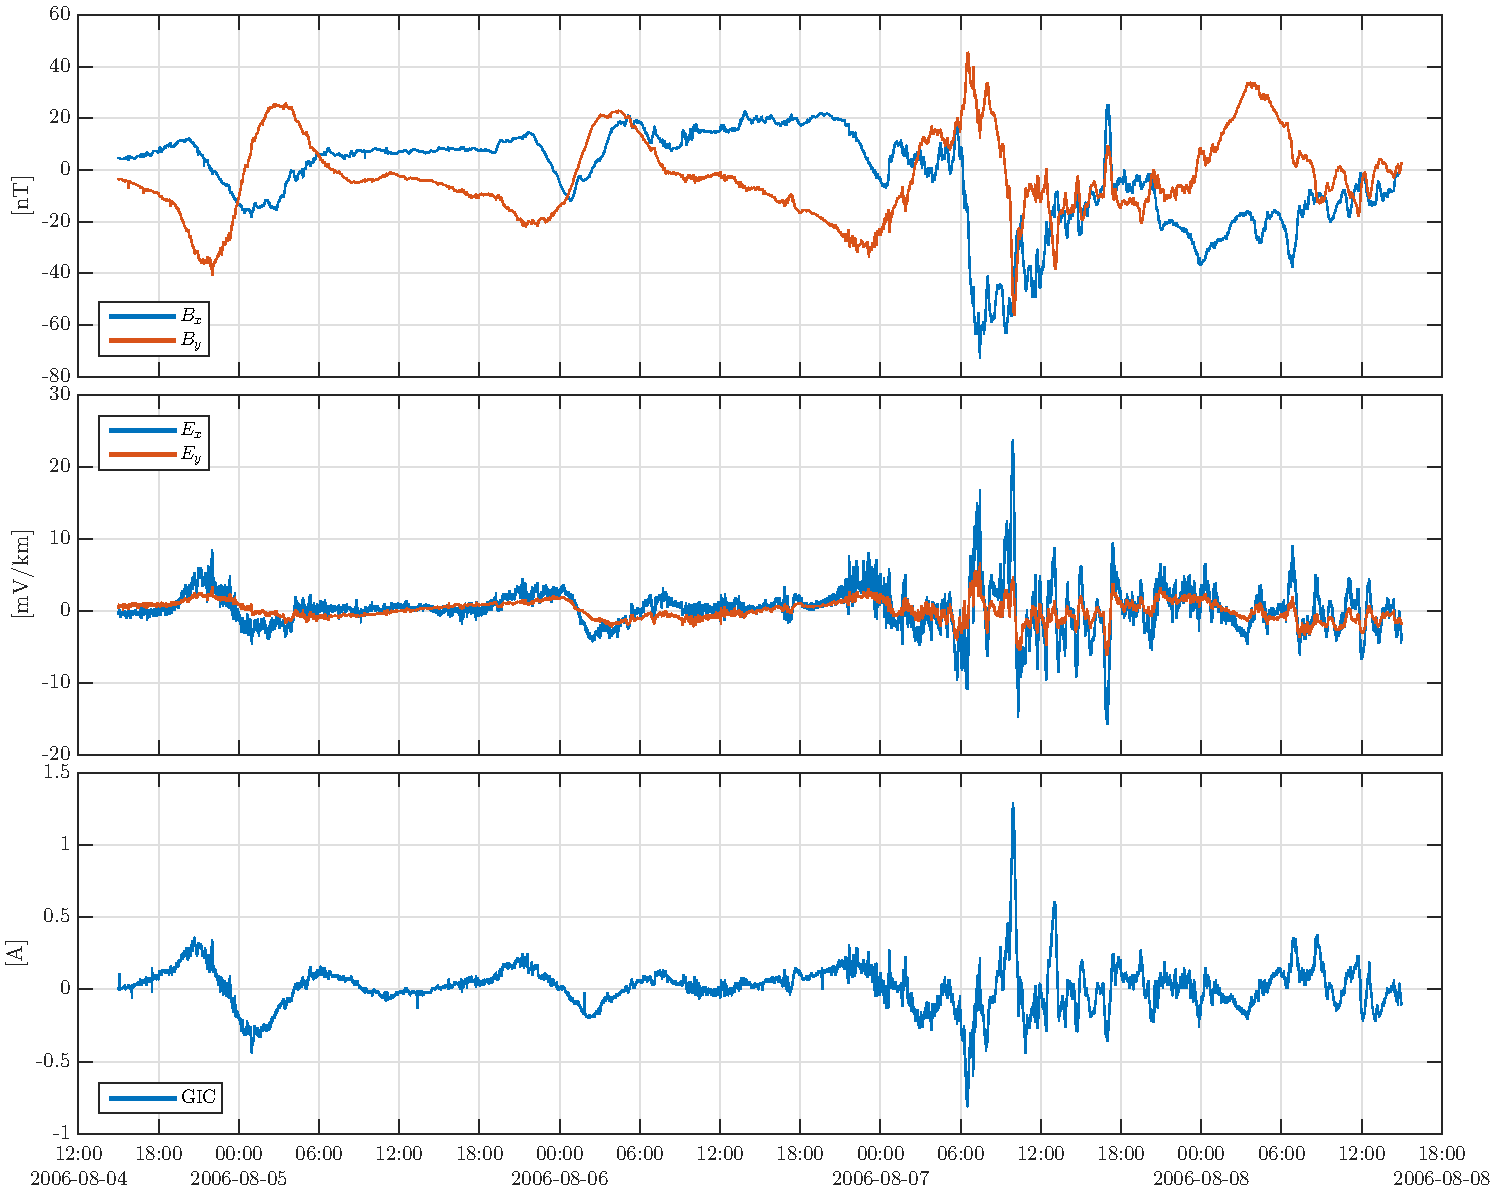
\includegraphics[width=\textwidth]{figures/plot_raw_All_20060805.pdf}
\caption{(Top) One-second-cadence geomagnetic field measured at the Memanbetsu Magnetic Observatory (MMB). (Middle) One-second-cadence geoelectric field measured at the Memanbetsu Magnetic Observatory (MMB) $\sim$10 km from the Memanbetsu substation. (Bottom) One-second-cadence GIC measurements measured in a grounded neutral point of a Y-connected three-phase transformer connected to a 187 kV bus at the Memanbetsu substation of the Hokkaido Power Co. The subscripts $x$, $y$, and $z$ correspond to North, East, and Downward, respectively.}
\label{sample}
\end{figure}

\begin{figure}[h]
\centering
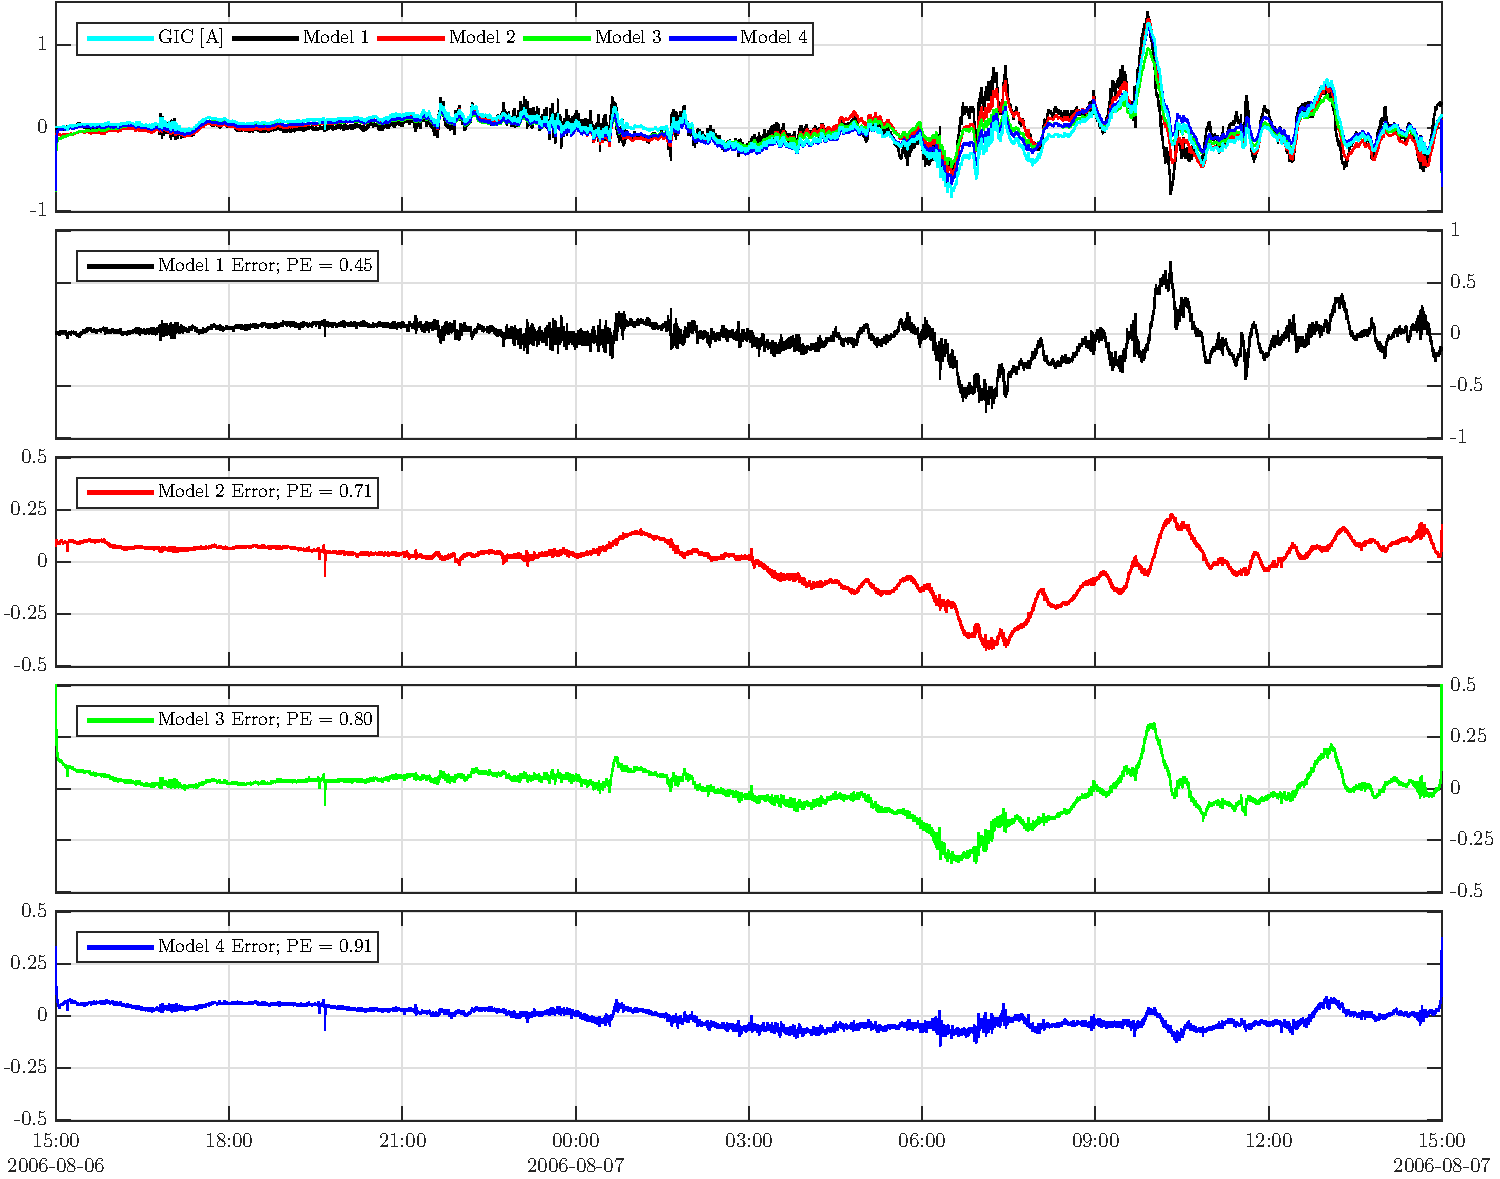
\includegraphics[width=\textwidth]{figures/plot_model_predictions-MeanModel-20060806T150000.pdf}
\caption{Out-of-sample model predictions (top) and predictions errors for a 1-day interval. Note that the scales for Models 2-4 differ from that for Model 1.}
\label{predictions}
\end{figure}

\begin{figure}[h]
\centering
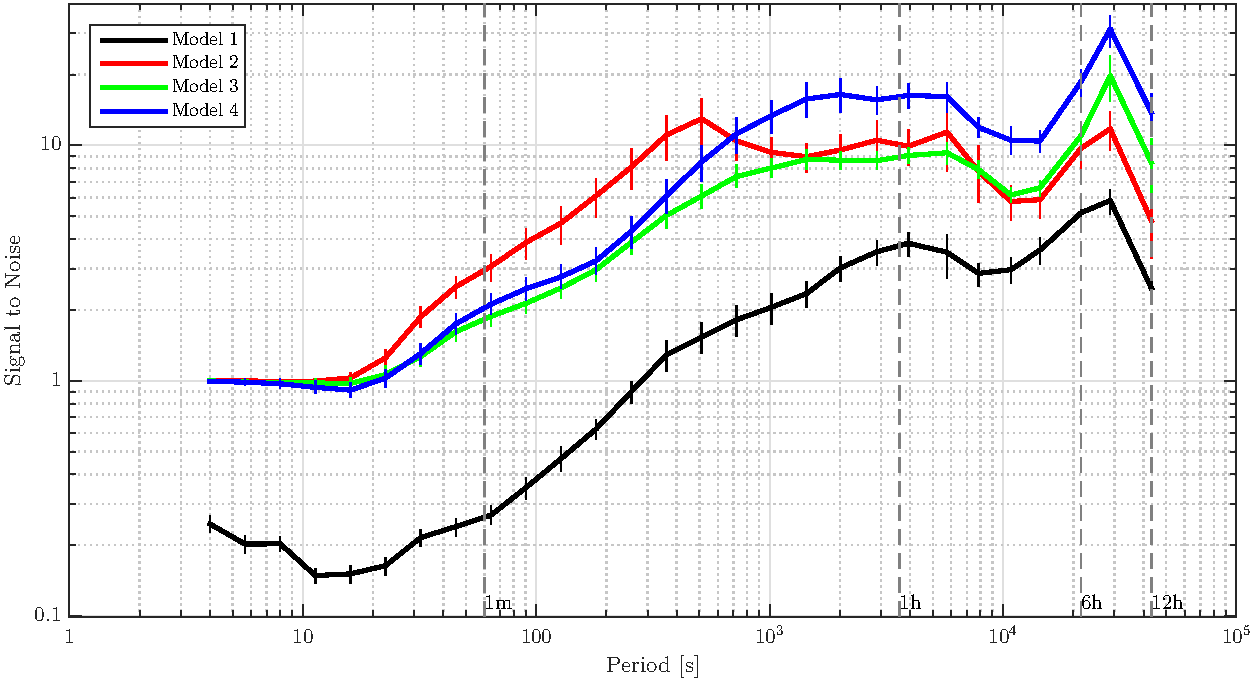
\includegraphics[width=\textwidth]{figures/plot_model_summary_SN-options-1.pdf}
\caption{Signal-to-noise ratios at the evaluation frequencies for the four models.}
\label{SN}
\end{figure}

\begin{figure}[h]
\centering
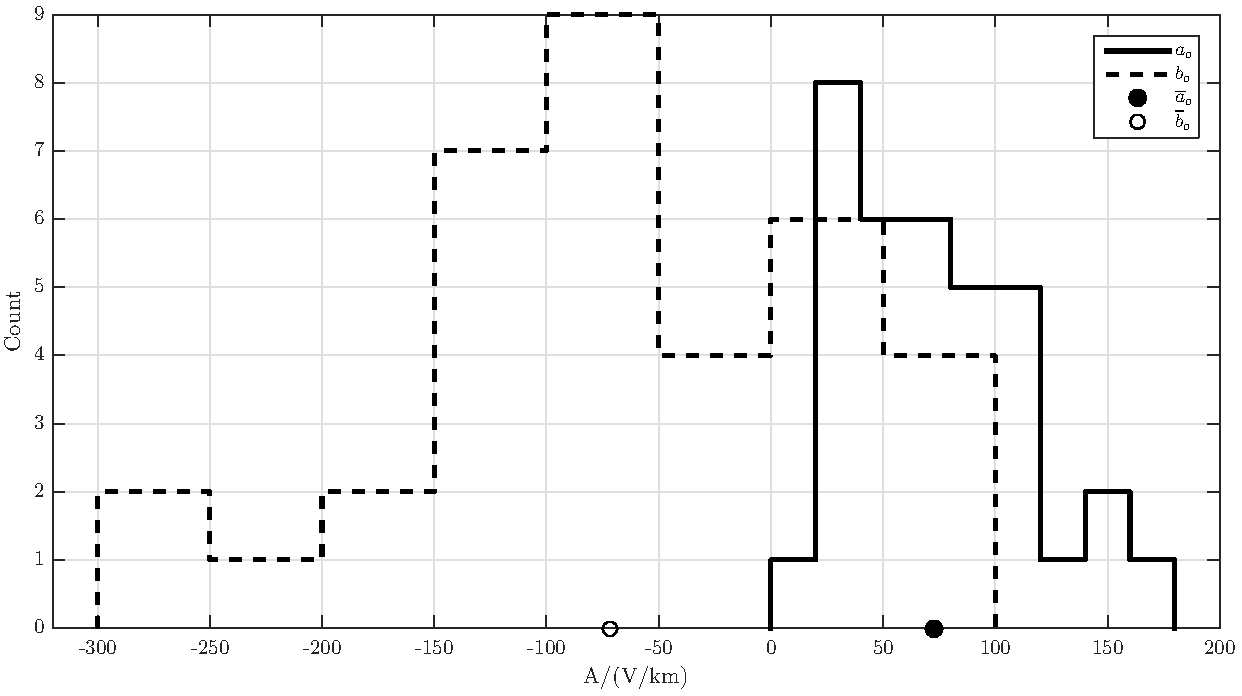
\includegraphics[width=\textwidth]{figures/plot_model_summary_aobo_histograms-options-1.pdf}
\caption{Distribution of parameters in Model 1. Each set of parameters were computed 35 times using one day of 1-second cadence data. The circle/dot on the horizontal axis indicates the average of each histogram: $a_o$ = 71.9 A/(V/km) and $b_o$ = -70.0 A/(V/km).}
\label{histogram}
\end{figure}

\begin{figure}[h]
\centering
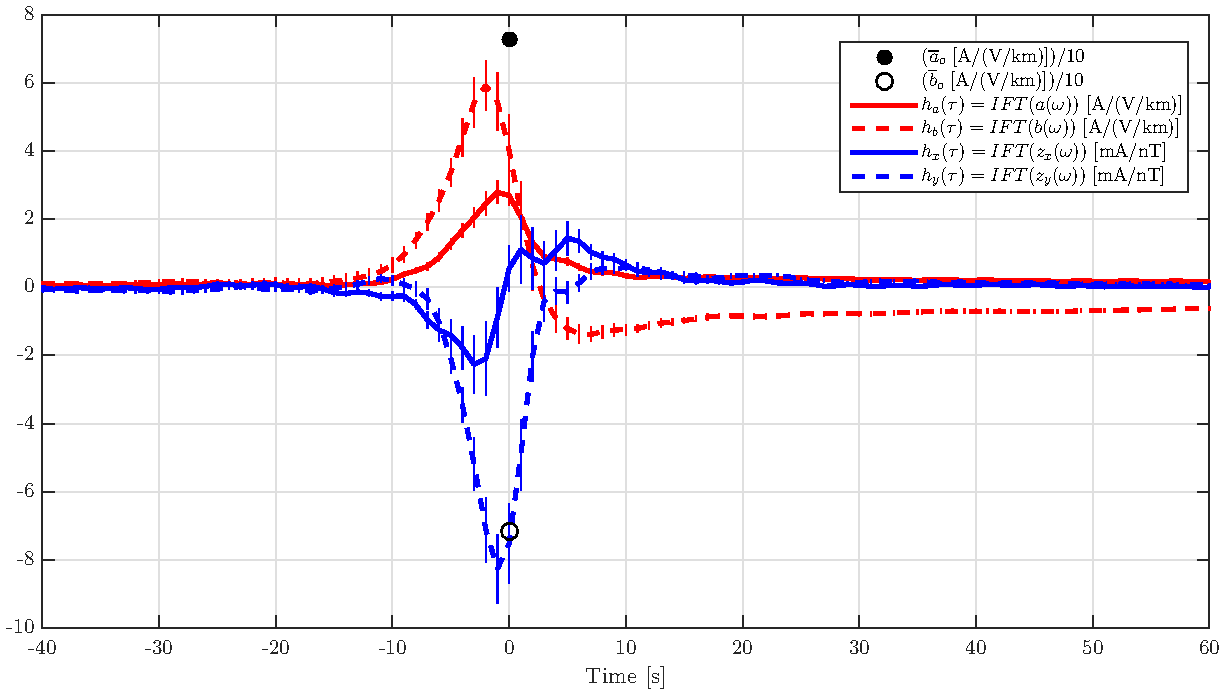
\includegraphics[width=\textwidth]{figures/plot_model_summary_H-options-1.pdf}
\caption{Impulse responses for Models 1, 2, and 4. The circles at $t = 0$ correspond to the impulse response for Model 1; the red/blue lines are the impulse responses for Model 2 and 4. The values of $a_o$ and $b_o$ have been scaled by a factor of 10 for readability.}
\label{H}
\end{figure}

\begin{figure}[h]
\centering
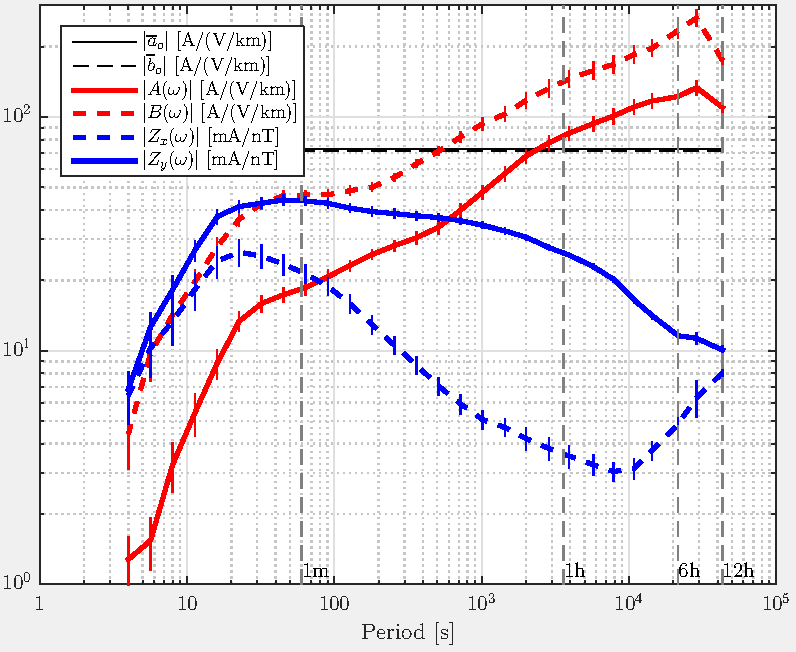
\includegraphics[width=\textwidth]{figures/plot_model_summary_Z-options-1.pdf}
\caption{Frequency domain transfer functions for Models 1-3. By definition, the frequency domain transfer functions for $A_o$ and $B_o$ are constant and equal to $a_o$ and $b_o$.}
\label{Z}
\end{figure}

\begin{figure}[h]
\centering
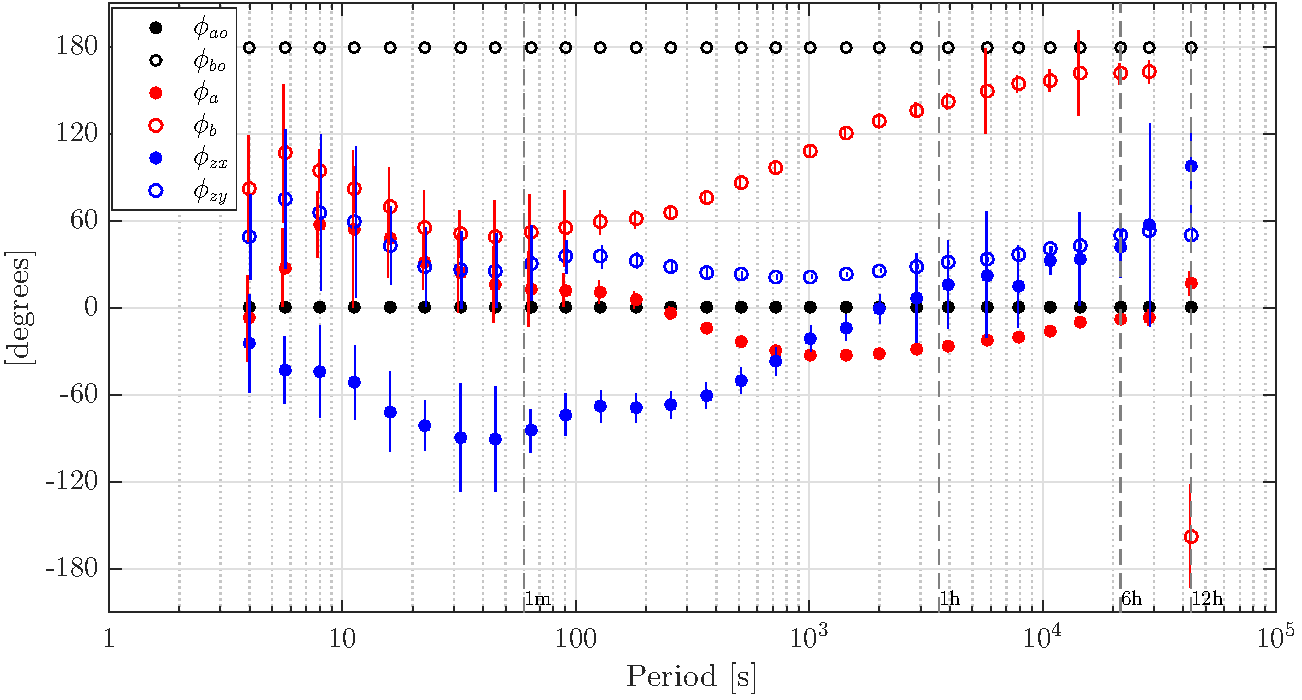
\includegraphics[width=\textwidth]{figures/plot_model_summary_Phi-options-1.pdf}
\caption{Frequency domain phase values for Models 1-3.}
\label{Phi}
\end{figure}


% Please use ONLY \citet and \citep for reference citations.
% DO NOT use other cite commands (e.g., \cite, \citeyear, \nocite, \citealp, etc.).
%% Example \citet and \citep:
%  ...as shown by \citet{Boug10}, \citet{Buiz07}, \citet{Fra10},
%  \citet{Ghel00}, and \citet{Leit74}.

%  ...as shown by \citep{Boug10}, \citep{Buiz07}, \citep{Fra10},
%  \citep{Ghel00, Leit74}.

\end{document}



More Information and Advice:

%% ------------------------------------------------------------------------ %%
%
%  SECTION HEADS
%
%% ------------------------------------------------------------------------ %%

% Capitalize the first letter of each word (except for
% prepositions, conjunctions, and articles that are
% three or fewer letters).

% AGU follows standard outline style; therefore, there cannot be a section 1 without
% a section 2, or a section 2.3.1 without a section 2.3.2.
% Please make sure your section numbers are balanced.
% ---------------
% Level 1 head
%
% Use the \section{} command to identify level 1 heads;
% type the appropriate head wording between the curly
% brackets, as shown below.
%
%An example:
%\section{Level 1 Head: Introduction}
%
% ---------------
% Level 2 head
%
% Use the \subsection{} command to identify level 2 heads.
%An example:
%\subsection{Level 2 Head}
%
% ---------------
% Level 3 head
%
% Use the \subsubsection{} command to identify level 3 heads
%An example:
%\subsubsection{Level 3 Head}
%
%---------------
% Level 4 head
%
% Use the \subsubsubsection{} command to identify level 3 heads
% An example:
%\subsubsubsection{Level 4 Head} An example.
%
%% ------------------------------------------------------------------------ %%
%
%  IN-TEXT LISTS
%
%% ------------------------------------------------------------------------ %%
%
% Do not use bulleted lists; enumerated lists are okay.
% \begin{enumerate}
% \item
% \item
% \item
% \end{enumerate}
%
%% ------------------------------------------------------------------------ %%
%
%  EQUATIONS
%
%% ------------------------------------------------------------------------ %%

% Single-line equations are centered.
% Equation arrays will appear left-aligned.

Math coded inside display math mode \[ ...\]
 will not be numbered, e.g.,:
 \[ x^2=y^2 + z^2\]

 Math coded inside \begin{equation} and \end{equation} will
 be automatically numbered, e.g.,:
 \begin{equation}
 x^2=y^2 + z^2
 \end{equation}


% To create multiline equations, use the
% \begin{eqnarray} and \end{eqnarray} environment
% as demonstrated below.
\begin{eqnarray}
  x_{1} & = & (x - x_{0}) \cos \Theta \nonumber \\
        && + (y - y_{0}) \sin \Theta  \nonumber \\
  y_{1} & = & -(x - x_{0}) \sin \Theta \nonumber \\
        && + (y - y_{0}) \cos \Theta.
\end{eqnarray}

%If you don't want an equation number, use the star form:
%\begin{eqnarray*}...\end{eqnarray*}

% Break each line at a sign of operation
% (+, -, etc.) if possible, with the sign of operation
% on the new line.

% Indent second and subsequent lines to align with
% the first character following the equal sign on the
% first line.

% Use an \hspace{} command to insert horizontal space
% into your equation if necessary. Place an appropriate
% unit of measure between the curly braces, e.g.
% \hspace{1in}; you may have to experiment to achieve
% the correct amount of space.


%% ------------------------------------------------------------------------ %%
%
%  EQUATION NUMBERING: COUNTER
%
%% ------------------------------------------------------------------------ %%

% You may change equation numbering by resetting
% the equation counter or by explicitly numbering
% an equation.

% To explicitly number an equation, type \eqnum{}
% (with the desired number between the brackets)
% after the \begin{equation} or \begin{eqnarray}
% command.  The \eqnum{} command will affect only
% the equation it appears with; LaTeX will number
% any equations appearing later in the manuscript
% according to the equation counter.
%

% If you have a multiline equation that needs only
% one equation number, use a \nonumber command in
% front of the double backslashes (\\) as shown in
% the multiline equation above.

% If you are using line numbers, remember to surround
% equations with \begin{linenomath*}...\end{linenomath*}

%  To add line numbers to lines in equations:
%  \begin{linenomath*}
%  \begin{equation}
%  \end{equation}
%  \end{linenomath*}



